% !TeX program = pdfLaTeX
\documentclass[12pt]{article}
\usepackage{amsmath}
\usepackage{graphicx,psfrag,epsf}
\usepackage{enumerate}
\usepackage{natbib}
\usepackage{textcomp}
\usepackage[hyphens]{url} % not crucial - just used below for the URL
\usepackage{hyperref}

%\pdfminorversion=4
% NOTE: To produce blinded version, replace "0" with "1" below.
\newcommand{\blind}{1}

% DON'T change margins - should be 1 inch all around.
\addtolength{\oddsidemargin}{-.5in}%
\addtolength{\evensidemargin}{-.5in}%
\addtolength{\textwidth}{1in}%
\addtolength{\textheight}{1.3in}%
\addtolength{\topmargin}{-.8in}%

%% load any required packages here


% Pandoc syntax highlighting
\usepackage{color}
\usepackage{fancyvrb}
\newcommand{\VerbBar}{|}
\newcommand{\VERB}{\Verb[commandchars=\\\{\}]}
\DefineVerbatimEnvironment{Highlighting}{Verbatim}{commandchars=\\\{\}}
% Add ',fontsize=\small' for more characters per line
\usepackage{framed}
\definecolor{shadecolor}{RGB}{248,248,248}
\newenvironment{Shaded}{\begin{snugshade}}{\end{snugshade}}
\newcommand{\AlertTok}[1]{\textcolor[rgb]{0.94,0.16,0.16}{#1}}
\newcommand{\AnnotationTok}[1]{\textcolor[rgb]{0.56,0.35,0.01}{\textbf{\textit{#1}}}}
\newcommand{\AttributeTok}[1]{\textcolor[rgb]{0.77,0.63,0.00}{#1}}
\newcommand{\BaseNTok}[1]{\textcolor[rgb]{0.00,0.00,0.81}{#1}}
\newcommand{\BuiltInTok}[1]{#1}
\newcommand{\CharTok}[1]{\textcolor[rgb]{0.31,0.60,0.02}{#1}}
\newcommand{\CommentTok}[1]{\textcolor[rgb]{0.56,0.35,0.01}{\textit{#1}}}
\newcommand{\CommentVarTok}[1]{\textcolor[rgb]{0.56,0.35,0.01}{\textbf{\textit{#1}}}}
\newcommand{\ConstantTok}[1]{\textcolor[rgb]{0.00,0.00,0.00}{#1}}
\newcommand{\ControlFlowTok}[1]{\textcolor[rgb]{0.13,0.29,0.53}{\textbf{#1}}}
\newcommand{\DataTypeTok}[1]{\textcolor[rgb]{0.13,0.29,0.53}{#1}}
\newcommand{\DecValTok}[1]{\textcolor[rgb]{0.00,0.00,0.81}{#1}}
\newcommand{\DocumentationTok}[1]{\textcolor[rgb]{0.56,0.35,0.01}{\textbf{\textit{#1}}}}
\newcommand{\ErrorTok}[1]{\textcolor[rgb]{0.64,0.00,0.00}{\textbf{#1}}}
\newcommand{\ExtensionTok}[1]{#1}
\newcommand{\FloatTok}[1]{\textcolor[rgb]{0.00,0.00,0.81}{#1}}
\newcommand{\FunctionTok}[1]{\textcolor[rgb]{0.00,0.00,0.00}{#1}}
\newcommand{\ImportTok}[1]{#1}
\newcommand{\InformationTok}[1]{\textcolor[rgb]{0.56,0.35,0.01}{\textbf{\textit{#1}}}}
\newcommand{\KeywordTok}[1]{\textcolor[rgb]{0.13,0.29,0.53}{\textbf{#1}}}
\newcommand{\NormalTok}[1]{#1}
\newcommand{\OperatorTok}[1]{\textcolor[rgb]{0.81,0.36,0.00}{\textbf{#1}}}
\newcommand{\OtherTok}[1]{\textcolor[rgb]{0.56,0.35,0.01}{#1}}
\newcommand{\PreprocessorTok}[1]{\textcolor[rgb]{0.56,0.35,0.01}{\textit{#1}}}
\newcommand{\RegionMarkerTok}[1]{#1}
\newcommand{\SpecialCharTok}[1]{\textcolor[rgb]{0.00,0.00,0.00}{#1}}
\newcommand{\SpecialStringTok}[1]{\textcolor[rgb]{0.31,0.60,0.02}{#1}}
\newcommand{\StringTok}[1]{\textcolor[rgb]{0.31,0.60,0.02}{#1}}
\newcommand{\VariableTok}[1]{\textcolor[rgb]{0.00,0.00,0.00}{#1}}
\newcommand{\VerbatimStringTok}[1]{\textcolor[rgb]{0.31,0.60,0.02}{#1}}
\newcommand{\WarningTok}[1]{\textcolor[rgb]{0.56,0.35,0.01}{\textbf{\textit{#1}}}}

% tightlist command for lists without linebreak
\providecommand{\tightlist}{%
  \setlength{\itemsep}{0pt}\setlength{\parskip}{0pt}}



\usepackage{booktabs}
\usepackage{longtable}
\usepackage{array}
\usepackage{multirow}
\usepackage{wrapfig}
\usepackage{float}
\usepackage{colortbl}
\usepackage{pdflscape}
\usepackage{tabu}
\usepackage{threeparttable}
\usepackage{threeparttablex}
\usepackage[normalem]{ulem}
\usepackage{makecell}
\usepackage{xcolor}

\begin{document}


\def\spacingset#1{\renewcommand{\baselinestretch}%
{#1}\small\normalsize} \spacingset{1}


%%%%%%%%%%%%%%%%%%%%%%%%%%%%%%%%%%%%%%%%%%%%%%%%%%%%%%%%%%%%%%%%%%%%%%%%%%%%%%

\if0\blind
{
  \title{\bf Detecting and Measuring Intervention Effects in R}

  \author{
        Alexis R. Santos \thanks{This research supported by the Social
Sciences Research Institute (SSRI) and the Population Research Institute
(PRI) at the Pennsylvania State University. Alexis R. Santos is a Social
Disparities Cluster faculty at SSRI. PRI is supported by a grant from
the Eunice Kennedy Shriver National Institute of Child Health and Human
Development (P2CHD041025), by the Pennsylvania State University, and by
SSRI.} \\
    Department of HDFS, Pennsylvania State University\\
     and \\     Mathew E. Hauer \\
    Department of Sociology, Florida State University\\
      }
  \maketitle
} \fi

\if1\blind
{
  \bigskip
  \bigskip
  \bigskip
  \begin{center}
    {\LARGE\bf Detecting and Measuring Intervention Effects in R}
  \end{center}
  \medskip
} \fi

\bigskip
\begin{abstract}
We provide a brief overview of two R packages that can be used to detect
and measure the causal effects of an intervention on a time series:
\textsf{CausalImpact} and \textsf{tsoutliers}. After an introduction of
both packages, and the data used in this paper we discuss the advantages
of these methods. During this explanation, we provide sample code and
discuss usage and results from a population-level dataset. Finally, we
highlight the similarities and differences of each package on modelling
causal effects.
\end{abstract}

\noindent%
{\it Keywords:} Outlier detection, Causal Inference, R software, time
series, causal methods
\vfill

\newpage
\spacingset{1.45} % DON'T change the spacing!

\hypertarget{introduction}{%
\section{Introduction}\label{introduction}}

The identification of causal effects (referred to as causal inference)
is a powerful motivation for social scientists
\citep{pearl2009causality}. Often, the identification of a causal
mechanism relies on comparisons to counterfactual control groups -- the
treatment group compared to a control group -- and the difference
between the two groups identifies the causal effect. ``Real world data''
rarely neatly bifurcate into treatment and control groups, especially
with longitudinal time series data, but the creation of ``synthetic''
counterfactual control groups in possible with both inductive and
abductive scientific approaches. Inductive analysis leverages knowledge
of an intervention to produce a synthetic control group and thus a
causal effect while abductive analysis identifies the potential effect
via outlier analysis and produces a counterfactual control group to
measure the size of the causal effect. This software review focuses on
detecting and measuring intervention effects and evaluates two
approaches available for conducting this analysis within the R software
framework \citep{rcore}.

Given the emergence and growing availability of intensive longitudinal
data (IDL), ecological momentary assessments (EMA), and other sources of
information such as social media activity or phone use, there is
increasing need to analyze time series, and isolate effects within the
phenomenon of interest \citep{McNeish, ram_screenomics_2020}. This paper
provides an overview of two packages in R that offer specific functions
to detect and measure intervention effects using both inductive and
abductive approaches: \textsf{CausalImpact}
\citep{brodersen2015inferring} and \textsf{tsoutlier} packages
\citep{tsoutliers}. In the following software review, we first describe
the illustrative data used in this paper, then provide sample code and
explore some of the options available within both packages. We conclude
this software review by comparing and discussing the results derived
from both functions.

\hypertarget{illustrative-data}{%
\section{Illustrative Data}\label{illustrative-data}}

We will use monthly death counts from the Puerto Rico Vital Statistics
System (PRVSS) to illustrate the functionality of the
\textsf{CausalImpact} and \textsf{tsoutliers} packages. The data contain
monthly aggregates of deaths for Puerto Rico between 2010 and 2018. Data
from the PRVSS has been used in many articles to estimate the excess
deaths following Hurricanes Irma and María
\citep{rivera_estimating_2018, sandberg2019all, santos2018use, SANTOSBURGOA2018e478, CruzCano}.
The original dataset includes individual records of each death occurring
in Puerto Rico between 2010 and 2018, with all the information collected
through the death certificate. The dataset employed in this Software
Review consists of aggregates for total deaths for every month between
March 2010 and December 2018 (Deaths), with corresponding month and year
identifiers. The dataset also includes a variable indicating the number
of observation each month represents (range = 1 - 106). This dataset
contains a total of 261,959 deaths distributed across 106 months
covering the month in which the 2010 census was collected (March 2010)
and the end of the year after Hurricanes Irma and María (December 2018).
Population estimates for these years are produced using the vital
statistics method and are in line with the population decline observed
in Puerto Rico 2010-onward \citep{santoslozada_puerto_2020}.
\textbf{\autoref{pr-table}} contains the first and last five
observations contained in the dataset.

\begin{longtable}[t]{rlrll}
\caption{\label{tab:unnamed-chunk-3}\textbf{Data set of monthly deaths in Puerto Rico, March 2010 to December 2018} \label{pr-table}}\\
\toprule
Obs & Month & Year & Deaths & Population Estimate\\
\midrule
1 & March & 2010 & 2,495 & 3,725,789\\
2 & April & 2010 & 2,298 & 3,713,097\\
3 & May & 2010 & 2,449 & 3,676,496\\
4 & June & 2010 & 2,405 & 3,683,013\\
5 & July & 2010 & 2,478 & 3,704,510\\
\addlinespace
102 & August & 2018 & 2,341 & 3,095,640\\
103 & September & 2018 & 2,233 & 3,079,240\\
104 & October & 2018 & 2,286 & 3,079,429\\
105 & November & 2018 & 2,353 & 3,082,268\\
106 & December & 2018 & 2,636 & 3,116,097\\
\bottomrule
\end{longtable}

\hypertarget{r-packages-for-detection-and-measuring-intervetions}{%
\section{R Packages for Detection and Measuring
Intervetions}\label{r-packages-for-detection-and-measuring-intervetions}}

\hypertarget{causalimpact-in-the-causalimpact-package}{%
\subsection{CausalImpact() in the CausalImpact
package}\label{causalimpact-in-the-causalimpact-package}}

The \textsf{CausalImpact} package developed by Kay H. Brodersen and
Alain Hauser implements a Bayesian approach to the estimation of causal
impact in time series and utilizes a classic, inductive approach to
measuring causal intervention effects \citep{brodersen2015inferring}. It
computes a causal impact as well as its duration using a pre- and
post-intervention approach. \textsf{CausalImpact} assumes that a time
series can be explained by a set of covariates which are not affected by
the intervention being measured. We use the previously introduced
dataset to demonstrate two of the multiple ways this package can be
used. First, we rely on an autoregressive model that uses the time
series past information to forecast a potential counterfactual and
second, we rely on the autoregressive model but controlling for
population size.

Usage of \textsf{CausalImpact()} is shown below with all arguments set
to the default.

\begin{Shaded}
\begin{Highlighting}[]
\FunctionTok{CausalImpact}\NormalTok{(}\AttributeTok{data =} \ConstantTok{NULL}\NormalTok{, }\AttributeTok{pre.period =} \ConstantTok{NULL}\NormalTok{, }\AttributeTok{post.period =} \ConstantTok{NULL}\NormalTok{, }
             \AttributeTok{model.args =} \ConstantTok{NULL}\NormalTok{,  }\AttributeTok{bsts.model =} \ConstantTok{NULL}\NormalTok{, }
             \AttributeTok{post.period.response =} \ConstantTok{NULL}\NormalTok{, }\AttributeTok{alpha =} \FloatTok{0.05}\NormalTok{)}
\end{Highlighting}
\end{Shaded}

A simple analysis using this function will require information in the
\texttt{data}, \texttt{pre.period}, and \texttt{post.period} arguments.
First, the \texttt{data} argument is the time series for which we want
to measure the intervention. The \texttt{pre.period} argument is the
period preceding the intervention, in this case the month in which the
Hurricane occurred. The \texttt{post.period} argument defines the
post-intervention window that defines the number of observations to be
considered after the intervention. Thus, some simple data processing is
required to conduct the analysis using \texttt{CausalImpact()}. We
produce a time series with the monthly death counts and need to specify
the pre- and post-intervention periods. This is accomplished with the
following code:

\begin{Shaded}
\begin{Highlighting}[numbers=left,,]
\NormalTok{deathspr }\OtherTok{\textless{}{-}}\NormalTok{ deaths\_pr}\SpecialCharTok{$}\NormalTok{Deaths}
\NormalTok{pop }\OtherTok{\textless{}{-}} \FunctionTok{log2}\NormalTok{(deaths\_pr}\SpecialCharTok{$}\NormalTok{Population\_Estimate)}
\NormalTok{data }\OtherTok{\textless{}{-}} \FunctionTok{cbind}\NormalTok{(deathspr) }
\NormalTok{data2 }\OtherTok{\textless{}{-}} \FunctionTok{cbind}\NormalTok{(deathspr, pop)}
\NormalTok{pre.period }\OtherTok{\textless{}{-}} \FunctionTok{c}\NormalTok{(}\DecValTok{1}\NormalTok{, }\DecValTok{90}\NormalTok{)}
\NormalTok{post.period }\OtherTok{\textless{}{-}} \FunctionTok{c}\NormalTok{(}\DecValTok{91}\NormalTok{, }\DecValTok{106}\NormalTok{)}
\end{Highlighting}
\end{Shaded}

The first and second line create a time series for the monthly deaths
and corresponding population estimates. The third lines create a
univariate time series object of just the deaths and the fourth line
creates a multivariate time series of both the deaths and population
estimates. The fifth and sixth lines are numeric values defining the
pre- and post-intervention period; these values are required to perform
the most basic analysis using \texttt{CausalImpact()}. How are the pre-
and post-intervention period defined? It comes from our understanding of
the data and determining when the intervention occurred. In our case,
the data contains observations for every month between 2000 and 2018. In
this data arrangement, September 2017 is the 91st observation. Thus, the
pre-intervention period is the period between observation 1 and 90, and
the post-intervention period is anything after that period (91-onward).
This is all the data manipulation and specifications we require to
conduct a simple \texttt{CausalImpact} analysis. The following code
illustrate the way to estimate the basic model and the numerous ways we
can explore the results:

\begin{Shaded}
\begin{Highlighting}[numbers=left,,]
\NormalTok{impact }\OtherTok{\textless{}{-}} \FunctionTok{CausalImpact}\NormalTok{(data, pre.period, post.period)}
\NormalTok{impact2 }\OtherTok{\textless{}{-}} \FunctionTok{CausalImpact}\NormalTok{(data2, pre.period, post.period)}

\NormalTok{impact}
\FunctionTok{summary}\NormalTok{(impact, }\StringTok{"report"}\NormalTok{)}
\FunctionTok{plot}\NormalTok{(impact)}
\end{Highlighting}
\end{Shaded}

\begin{Shaded}
\begin{Highlighting}[]
\NormalTok{impact }\OtherTok{\textless{}{-}} \FunctionTok{CausalImpact}\NormalTok{(data, pre.period, post.period)}
\NormalTok{impact2 }\OtherTok{\textless{}{-}} \FunctionTok{CausalImpact}\NormalTok{(data2, pre.period, post.period)}
\end{Highlighting}
\end{Shaded}

The above code stores the output from \texttt{CausalImpact()} in an
object called \texttt{impact} for the model that does not consider
population size and \texttt{impact2} for the one with controls for
population size. The function includes the three main arguments
described above. The results can be explored in three ways: (1) by
examining the raw output as in \textbf{\autoref{impact}}, (2) by asking
R to produce a brief report (\textbf{\autoref{report}}), and (3) by
producing a visualization of the intervention effect
(\textbf{\autoref{plots}}).

By simply calling the \texttt{impact} object which contains the output
from the \texttt{CausalImpact()} function, the package provides the
Actual and Predicted averages and cumulative counts, and shows the
absolute and relative effect of the intervention. These pieces of
information are accompanied by their corresponding measures of error and
95\% intervals. Here we can see the absolute cumulative effect of
Hurricane María is 1,155 deaths with a p-value of 0.04805.

\begin{figure}
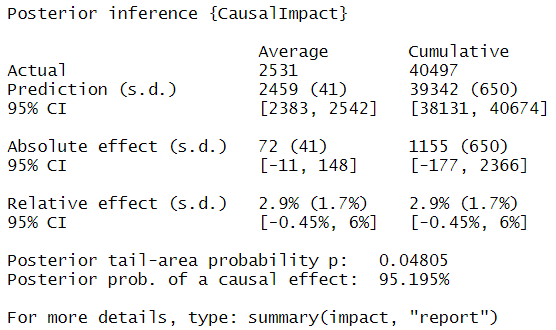
\includegraphics[width=1\linewidth]{../MainDocument/Capture} \caption{\textbf{Raw output from the object created by the CausalImpact() function.}\label{impact}}\label{fig:unnamed-chunk-8}
\end{figure}

By using the \texttt{summary(impact,\ "report")} function, we request a
narrative summary of the analysis. Note, that simply asking for a
summary without specifying the report section will yield the same
results as the second line (ie using \texttt{summary(impact)}). In
\textbf{\autoref{report}} we present the full text that comes from
report which is a comprehensive analysis of the intervening being
analyzed. The report is divided in five subsections. Section 1 describes
what happened during the post-intervention period and present a brief
overview of the causal effect. Section 2 aggregates the data from the
post-intervention period and provides a brief overview of what occurred
and what would have occurred absent the intervention. Section 3
transforms the results described in Section 2 into relative terms, in
this case the percent increase observed in the death counts and the
corresponding 95\% interval. Section 4 summarizes the effect of the
intervention, indicates whether there is a significant effect, and asks
the researcher to compare the absolute effect with the goal of the
intervention. Section 5 describes the probability that the effect
happened at random with a corresponding p-value. The concluding sentence
asserts whether the causal effect can be considered statistically
significant. The results presented in this report indicate that
Hurricane María constituted a significant intervention regarding the
number of deaths and that it is highly unlikely that this occurred by
chance.

\begin{figure}
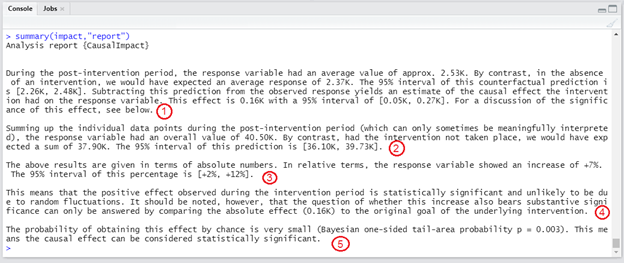
\includegraphics[width=1\linewidth]{../MainDocument/Picture1} \caption{\textbf{CausalImpact narrative report resulting from the assessment of mortality following Hurricane María.}\label{report}}\label{fig:unnamed-chunk-9}
\end{figure}

\begin{Shaded}
\begin{Highlighting}[numbers=left,,]
\NormalTok{impact.plot }\OtherTok{\textless{}{-}}  \FunctionTok{plot}\NormalTok{(impact) }\SpecialCharTok{+}  
  \FunctionTok{theme\_bw}\NormalTok{(}\AttributeTok{base\_size =} \DecValTok{12}\NormalTok{) }\SpecialCharTok{+}
  \FunctionTok{labs}\NormalTok{(}\AttributeTok{title =} \StringTok{"Without Population Controls (univariate)"}\NormalTok{, }
       \AttributeTok{x =}\StringTok{"Time"}\NormalTok{, }
       \AttributeTok{y =} \StringTok{"Deaths"}\NormalTok{)}

\NormalTok{impact.plot2 }\OtherTok{\textless{}{-}} \FunctionTok{plot}\NormalTok{(impact2) }\SpecialCharTok{+}  
  \FunctionTok{theme\_bw}\NormalTok{(}\AttributeTok{base\_size =} \DecValTok{12}\NormalTok{) }\SpecialCharTok{+}
  \FunctionTok{labs}\NormalTok{(}\AttributeTok{title =} \StringTok{"With Population Controls (multivariate)"}\NormalTok{, }
       \AttributeTok{x =} \StringTok{"Time"}\NormalTok{, }
       \AttributeTok{y =} \StringTok{"Deaths"}\NormalTok{)}

\NormalTok{ggpubr}\SpecialCharTok{::}\FunctionTok{ggarrange}\NormalTok{(impact.plot, }
\NormalTok{                  impact.plot2, }
                  \AttributeTok{ncol=}\DecValTok{1}\NormalTok{, }
                  \AttributeTok{nrow=}\DecValTok{2}\NormalTok{) }\CommentTok{\#Combines both graphs }
\end{Highlighting}
\end{Shaded}

The third and final way we can assess the effect of the intervention is
by visually examining the time series, the effect estimates, and the
cumulative effect. The \texttt{CausalImpact} package is compatible with
the basic plot functions included in R. The fourth line in the previous
code uses \texttt{plot()} in combination with the impact object to
produce a plot with three panels. These panels include: (1) the original
time series (black line) with the expected time series in light blue,
(2) the effect estimates for the post-intervention period, and (3) the
cumulative effect. The timing of the intervention is represented by a
dashed-vertical line in each of the panels. Both the pointwise and
cumulative estimates are accompanied by corresponding 95\% intervals.
The visualization indicates that mortality on and after September 2017
exceeded the expected range and that this effect was sustained for a
couple of months after Hurricane María. In \textbf{\autoref{plots}}, we
present the resulting plots for both impact analyses described above. We
combined the basic plot function with functions from the
\texttt{ggplot2} and \texttt{ggpubr} packages. These figures were
produced using the following code:

\begin{figure}
\centering
\includegraphics{MainDocument_files/figure-latex/unnamed-chunk-11-1.pdf}
\caption{\textbf{Visualization of CausalImpact results without and with controls for population size as univariate and multivariate time series.}
\label{plots}}
\end{figure}

\hypertarget{tso-in-the-tsoutliers-package}{%
\subsection{\texorpdfstring{\texttt{tso()} in the \texttt{tsoutliers}
package}{tso() in the tsoutliers package}}\label{tso-in-the-tsoutliers-package}}

The \texttt{tsoutliers} package \citep{tsoutliers} implements a
mathematical approach for the automatic detection of outliers in both
univariate and multivariate time series originally formulated by Chen
and Liu in 1993 \citep{chen1993joint}. In contrast to the
\texttt{CausalImpact} package which uses an inductive approach to
estimating the magnitude of a causal effect, the \texttt{tsoutliers}
package uses an abductive approach for both finding and estimating
causal effects. \texttt{CausalImpact} requires ex-post knowledge of an
intervention to measure the magnitude of the effect.
\texttt{tsoutliers}, by virtue of its abductive approach, does not
require ex-post knowledge as the algorithm searches the time series for
anomalous behavior and the cause of the effect is reasoned ex-post.

Time series are affected by exogenous factors and the effects are felt
differently across the phenomenon of our interest. Aside from detecting
outliers within a time series, the \texttt{tso()} function offers
insights about the effect being captured when an outlier is detected. By
default, three types of outliers detected are:

\begin{enumerate}
\def\labelenumi{\arabic{enumi}.}
\tightlist
\item
  Additive outliers (AO) - isolated large or small values within the
  time series,
\item
  Level shifts (LS) - a change in the average levels with the
  observations following the outlier shifting accordingly. This change
  may be due to seasonality, but has the distinctive feature of the
  change being more permanent, and
\item
  Temporary or transient changes (TC) - similar to LS but the effect of
  the outlier reduces over subsequent observations. Eventually, the
  values return to the levels observed prior to the outlier.
\end{enumerate}

The two additional outliers featured in this package are: 4. Innovative
outliers (IO) - outliers that derive from innovation in the data
generating process that affects all subsequent observations, and 5.
Seasonal level shifts (SLS) - similar to LS but they occur at some point
and reoccur every year (time window) at the same season and its effect
affects the subsequent seasons.

The \texttt{tso()} function iteratively uses ARIMA models to 1) identify
potential outliers or anomalies and 2) refit the ARIMA with the outliers
removed to produce a counter-factual time series. A detailed discussion
of these outliers and the detection algorithm is available in extant
literature
\citep{chen1993joint, tsoutliers, asghar2017analysis, burman1988outliers}.

Usage of \texttt{tso()} is shown below with all arguments set to the
default:

\begin{Shaded}
\begin{Highlighting}[]
\FunctionTok{tso}\NormalTok{(y, }\AttributeTok{xreg =} \ConstantTok{NULL}\NormalTok{, }\AttributeTok{cval =} \ConstantTok{NULL}\NormalTok{, }\AttributeTok{delta =} \FloatTok{0.7}\NormalTok{, }\AttributeTok{types =} \FunctionTok{c}\NormalTok{(}\StringTok{"AO"}\NormalTok{, }\StringTok{"LS"}\NormalTok{, }\StringTok{"TC"}\NormalTok{), }
    \AttributeTok{maxit =} \DecValTok{1}\NormalTok{, }\AttributeTok{maxit.iloop =} \DecValTok{4}\NormalTok{, }\AttributeTok{maxit.oloop =} \DecValTok{4}\NormalTok{, }\AttributeTok{cval.reduce =} \FloatTok{0.14286}\NormalTok{,    }
    \AttributeTok{discard.method =} \FunctionTok{c}\NormalTok{(}\StringTok{"en{-}masse"}\NormalTok{, }\StringTok{"bottom{-}up"}\NormalTok{), }\AttributeTok{discard.cval =} \ConstantTok{NULL}\NormalTok{, }
\NormalTok{    remove.method, remove.cval, }\AttributeTok{tsmethod =} \FunctionTok{c}\NormalTok{(}\StringTok{"auto.arima"}\NormalTok{, }\StringTok{"arima"}\NormalTok{),   }
    \AttributeTok{args.tsmethod =} \ConstantTok{NULL}\NormalTok{, }\AttributeTok{logfile =} \ConstantTok{NULL}\NormalTok{, }\AttributeTok{check.rank =} \ConstantTok{FALSE}\NormalTok{)}
\end{Highlighting}
\end{Shaded}

Most of the default arguments pertain to the creation of the arima
models and will work well for most exploration of outliers. Here, we use
the \texttt{y}, \texttt{types}, and \texttt{xreg} arguments to determine
whether the number of deaths following Hurricane María is considered an
outlier, and if so, the type and magnitude of the outlier. In addition,
we explore whether the results change when we control for population
size. First, the \texttt{y} argument is the time series of interest and
must be a time series object. Rarely, R will import time series data as
a time series object, rather than a dataframe, so most analyses require
simple data processing to convert the data into a format compatible with
\texttt{tso()}. For analyzing a multivariate time series using the
\texttt{xreg} argument, the dataformat is slightly different and must be
in the form of a matrix or array. After importing the data, we transform
the information into a time series using the \texttt{ts()} function
available through the \texttt{stats} library, as follows:

\begin{Shaded}
\begin{Highlighting}[numbers=left,,]
\NormalTok{Deaths\_ts }\OtherTok{\textless{}{-}}\NormalTok{ stats}\SpecialCharTok{::}\FunctionTok{ts}\NormalTok{(deaths\_pr}\SpecialCharTok{$}\NormalTok{Deaths, }\AttributeTok{frequency=}\DecValTok{1}\NormalTok{) }
\NormalTok{Popula\_ts }\OtherTok{\textless{}{-}}\NormalTok{ deaths\_pr}\SpecialCharTok{$}\NormalTok{Population\_Estimate}
\end{Highlighting}
\end{Shaded}

The first line creates a time series for the monthly deaths from 2010
until 2018 and the second one creates a time series object for the
corresponding monthly population estimates. This information was
contained within the dataset we imported in the illustrative data
section (see \textbf{\autoref{pr-table}}). This is all the data
manipulation required to have the data in a format that is familiar to
the \texttt{tso()} function.

The essential arguments for \texttt{tso()} are the time series of
interest for detecting outliers, the type of outliers to detect, and
potentially a control variable or variables (\texttt{xreg}). We start
with a simple model that only considers the monthly death counts
(\texttt{y}), specifying the detection for the three default types of
outliers: AO, LS, and TC. The models are estimated using the following
code:

\begin{Shaded}
\begin{Highlighting}[numbers=left,,]
\NormalTok{analysis }\OtherTok{\textless{}{-}} \FunctionTok{tso}\NormalTok{(Deaths\_ts, }\AttributeTok{types=}\FunctionTok{c}\NormalTok{(}\StringTok{"AO"}\NormalTok{,}\StringTok{"LS"}\NormalTok{,}\StringTok{"TC"}\NormalTok{))}

\NormalTok{analysis2 }\OtherTok{\textless{}{-}} \FunctionTok{tso}\NormalTok{(}\AttributeTok{y=}\NormalTok{Deaths\_ts, }\AttributeTok{xreg =}\NormalTok{ Popula\_ts, }\AttributeTok{types=}\FunctionTok{c}\NormalTok{(}\StringTok{"AO"}\NormalTok{,}\StringTok{"LS"}\NormalTok{,}\StringTok{"TC"}\NormalTok{))}
\end{Highlighting}
\end{Shaded}

The above code stores the output from \texttt{tso()} in two separate
objects called \texttt{analysis} for the univariate time series and
\texttt{analysis2} for the multivariate. The difference between both
analyses is the inclusion of population estimates to account for changes
in population size. We access the results by: (1) looking at the output
in table form (\textbf{\autoref{tso-table}}) or (2) through data
visualization (\textbf{\autoref{tso-plot}}). To examine the output table
one must simply write the name of the object where the results are
stored in the console. The output includes the type of outlier detected,
the observation id, the estimated excess, and the t-statistic associated
with the outlier.

\begin{longtable}[t]{llrrrr}
\caption{\label{tab:unnamed-chunk-15}\textbf{Outlier detection for monthly deaths for Puerto Rico, 2010-2018 without (univariate) and with (multivariate) controls for population size.} 'type' describes the type of outlier, 'ind' refers to the time index of the detected outlier, 'time' refers to the specified time, 'coefhat' is the size of the detected outlier, and 'tstat' is the critical value of the detected outlier. \label{tso-table}}\\
\toprule
Analysis & type & ind & time & coefhat & tstat\\
\midrule
Univariate & TC & 91 & 91 & 597.166 & 4.71754\\
Multivariate (population size) & TC & 91 & 91 & 682.438 & 5.16327\\
\bottomrule
\end{longtable}

In both instances, the model identified September 2017 (time indexed
value 91) as a temporary change (TC) outlier. This tells us that the
number of deaths detected in the month of Hurricane María exceeded the
expected levels and that this effect was not constrained to that month,
it continued affecting Puerto Rico for subsequent months until the point
the number of deaths returned to expected levels. In this case,
\texttt{coefhat} represents the excess deaths observed in this month.
The univariate model indicates that there were 597 deaths in excess of
historical patterns in that month and the multivariate analysis
accounting for population size indicates that 682 deaths occurred in
excess of expected levels.

This outlier was classified as a TC type of outlier; this means the
effect of the hurricane is lingered for some subsequent periods. To
better understand the impact of the Hurricane and its diminishing
effects, it is best to visualize the outlier in comparison to the time
series and how this observation, and subsequent ones, deviate from the
expected pattern. The tsoutlier package is compatible with the basic
plotting functions. To produce a visual representation of the time
series and the outlier effects we use \texttt{plot()}. For purposes of
brevity, we show the visualization of the multivariate model that
controls for population size.

We simply ask R to plot the object where the output is stored:

\begin{Shaded}
\begin{Highlighting}[]
\FunctionTok{plot}\NormalTok{(analysis2)}
\end{Highlighting}
\end{Shaded}

\begin{figure}
\centering
\includegraphics{MainDocument_files/figure-latex/unnamed-chunk-16-1.pdf}
\caption{\textbf{Plot of the tso function that considers population size through the xreg argument.}
Detecting one outlier in September 2017 (red dot) with a diminishing
effect in the following months until the time series converges towards
the expected levels based on pre-Hurricane María patterns represented in
the outlier effects panel. \label{tso-plot}}
\end{figure}

\hypertarget{comparison-of-the-tsoutlier-and-causlimpact-packages}{%
\subsection{\texorpdfstring{Comparison of the \texttt{tsoutlier} and
\texttt{CauslImpact}
packages}{Comparison of the tsoutlier and CauslImpact packages}}\label{comparison-of-the-tsoutlier-and-causlimpact-packages}}

Previous studies that employ a time series approach to estimate excess
deaths in Puerto Rico have estimated the excess deaths in September 2017
to be: 574 (95\% C.I. 515-630), 449 (95\% C.I. 377-527), and 459 (95\%
C.I. 425-293)
\citep{rivera_estimating_2018, santos2018differential, santos2018use}.
The results derived from both the \texttt{CausalImpact} and
\texttt{tsoutliers} packages are consistent or close to these estimates.
Furthermore, without programming in September 2017 as the date of the
hurricane, the \texttt{tso} function correctly identifies September 2017
as an outlier when compared to the expected counts.

While the results of both functions are similar to each other and to
published results, the process and formulation of the approach differ.
As stated above, the packages utilize different logical approaches to
identifying and estimating causal effects. \texttt{CausalImpact} uses a
more classical, inductive approach to identify effects and if one knows
the date of an intervention, the \texttt{CausalImpact} package might be
a reasonable choice. However, sometimes the date of an intervention is
unknown. Take for instance the COVID-19 pandemic, the onset of the
pandemic is not knowable for all states or countries. If one were to try
and identify the excess mortality of the pandemic, the
\texttt{tsoutliers} package might be a more reasonable choice. Both
functions have some form of significance testing. \texttt{tso()}
provides a t-statistic that corresponds to the detected outlier while
the \texttt{CausalImpact} function provides a p-value corresponding to a
Bayesian-one sided tail area probability. Finally, both functions
provide a way of visually examining the time series and the resulting
analysis. Both methods allow us to conclude that the Hurricane María
caused deaths in excess of expected levels as established in the extant
literature \citep{sandberg2019all}.

\hypertarget{discussion}{%
\section{Discussion}\label{discussion}}

There is a growing interest and need to assess the causal effects of
interventions \citep{pearl2009causality} and the \texttt{tsoutliers} and
\texttt{CausalImpact} packages provide avenues to identify causal
effects for time series data.

Due to the different logical approaches to estimating causality, the
packages both similar and different data requirements. Both packages
require a time series for which detection and measurement of a causal
effect are desired and both packages are compatible with univariate and
multivariate time series. For \texttt{tso()} multivariate times series
are included by specifying the \texttt{xreg} argument. To incorporate
controls within the \texttt{CausalImpact} approach, they need to be
included in the data matrix. This matrix should be structured in a way
that the first column corresponds to the time series of interest, and
the subsequent columns are the controls. Despite slight differences in
both mathematical formulation and empirical approach, both methods
produce similar results. Only the \texttt{CausalImpact} approach
requires additional information about the timing of an intervention, the
\texttt{tsoutliers} package searches for the intervention. This is a
direct result of the objective of each function, while
\texttt{tsoutliers} is a more powerful detection tool and
\texttt{CausalImpact} might be better suited to measure an intervention
effect when knowledge of the specific timing of an intervention is
available.

The \texttt{tso()} function does not calculate the cumulative effect of
a detected outlier but this can be remedied with basic arithmetic. To
measure the cumulative effect, we subtract the expected values from the
observed ones after the outlier is detected. The summation of these
differences is the cumulative effect of the intervention. While simple
in coding, researchers need to be careful not to include effects that
correspond to another outlier into the total. In our illustrative
example, only one outlier was detected so this is not an issue. However,
the situation becomes more complex when multiple outliers are detected
and for instances where these outliers may have an effect in subsequent
periods or when we observe a shift in the time series. Thus, estimating
cumulative effects is a process that should be performed with caution
and after a careful examination of the results.

Visualizations with both packages are easy to produce and interpret.
These are produced using the \texttt{plot()} function which is part of
the original or base graphics functions included with R. When plotting
the results from \texttt{tso()}, a two-panel graph is produced where the
upper panel presents the time series and highlights any outliers
detected. The lower panel provides insights as to how far the outlier is
from the expected value and for how long this effect lasts. How long did
the effect last? The \texttt{tso()} can detect isolated points,
concentrated effects, or significant shifts in the time series. Thus, it
provides a simple, yet elegant visualization that allows following the
effect across time. In the case of the \texttt{CausalImpact()}
visualization, the plot function produces three panels, modifiable with
code. The first panel, labeled original, is similar to the upper panel
produced with \texttt{tso()} and it shows the time series and the
expected values. The second panel is similar to the lower panel produced
with \texttt{tso()} and it shows the effect estimates for each
post-intervention observation. The third panel is unique to
\texttt{CausalImpact()} and consists of the cumulative effect of the
intervention. The key distinction between both visualizations is that
\texttt{CausalImpact()} includes a dashed-vertical line representing the
start of the post-intervention period. In our code, we also provide
examples that combine the initial plots with functions from the
\texttt{ggplot2} and \texttt{ggpubr} packages to put titles and axes
titles in both figures, and to join them into one data visualization.
Although this last comment deals with the aesthetics of visualization,
and not with the results, we highlight the possibility of modifying the
visualization, which can be useful when researchers are interested in
producing publication-ready figures.

In closing, both packages are similar in that they produce consistent
estimates following an intervention. However, they offer different
insights into the intervention that users should be aware of. The
\texttt{tsoutliers} package is better suited for analyses where we are
interested in \emph{detecting} potential intervention effects within a
time series. On the other hand, the \texttt{CausalImpact} package is
better suited for analyses where the timing of the intervention is
known. While other approaches exist, we see a fruitful and promising
avenue for the use of both functions to detect and measure intervention
effects when time series are available. Both packages have their
strengths and weaknesses, but they can be used to perform both inductive
and abductive assessments of interventions.

\bibliographystyle{agsm}
\bibliography{bibliography.bib}


\end{document}
